\documentclass[../main.tex]{subfiles}
%\graphicspath{{\subfix{./images/}}} %Does not work...

\newcommand\sbWidth{\textwidth} %Use this to set the width of all images simultaneously!

\begin{document}
\section{Problem Solving Approach and System Design}\label{prototypes}
After brainstorming various solutions, the next step in the design process was to decide upon a prototype solution. The process to decide upon a final solution is quite complicated, as a variety of factors must be considered in order for the prototype to fit our project scope \emph{and} coincide with the mission and vision statements of the team.\par
The selection, analysis, and formulation of this prototype consists of the following steps:\par
\begin{singlespace}
\begin{enumerate}
    \item Analyze the proposed solutions. Consider the solution's scope, feasability, and alignment with the group's direction thus far.
    \item Decide upon a solution, using a \textbf{decision matrix} to assist in the selection process
    \item Once a solution has been selected, take time to expand upon the solution and analyze the solution's constituent components.
    \item Present the solution in an easy-to-understand and quickly iterated manner to rapidly tune the design for final production.
\end{enumerate}
\end{singlespace}

\newpage
\subsection{Analysis of proposed solutions}
In section \ref{designProcess}, the team created multiple solutions that they believed would satisfy our project's goals. All of these solutions satisfied a portion of what we attempt to solve in this publication. However, only one solution, or a combination of multiple, will make it to the prototyping phase. Substantial effort was invested into the creation of the proposed solutions in order to provide the prototyping phase a more concise and accurate selection process - as opposed to having \emph{obviously} poor solutions in the mix. The nature of our problem statment provides a variety of options that are entierly feasable as a design solution, and this can be seen in the resultant products from section \ref{designProcess}.\par

\subsection{Selection of the prototype}
Due to the careful consideration of our solution design, it was quite easy to then utilize a both common and extremely powerful tool to arrive at our prototype route: the decision matrix. As established Penn State engineers, we were familiar with a method from a previous EDSGN 100 class that we agreed could work well for the task at hand. We ported the template to our purposes and discussed our "selection criteria" and their significance/weight. These criteria were the factors that we considered most relevant in determining the best solution, such as safety, cost, associated risk, etc. \par

The following page shows the resultant selection matrix indicating the best (green) and worst (red) solutions. Scores for each category were aggregated via simple mean value between independent group member assessment.\par

\newpage
\subsubsection{Prototype Selection Matrix}
\noindent For easy reference in the solution matrix, below can be found a short description of each solution:
\begin{singlespace}
\begin{description}
    \item[Solution \#1:] A privatized aircraft hangar supplied by the customer for use by solely the customer.
    \item[Solution \#2:] Airport or FBO-owned airport hangars for use by multiple companies wishing to operate EA out of the airport.
    \item[Solution \#3:] Development of a subsidy package for local/state/federal government funding of infrastructure installation.
    \item[Solution \#4:] A distributed power generation, storage, and distribution system for charging EA.
    \item[Solution \#5:] A large-scale power generation system with capability for on-grid power transfer.
\end{description}
\end{singlespace}

\begin{figure}
\centering
\fbox{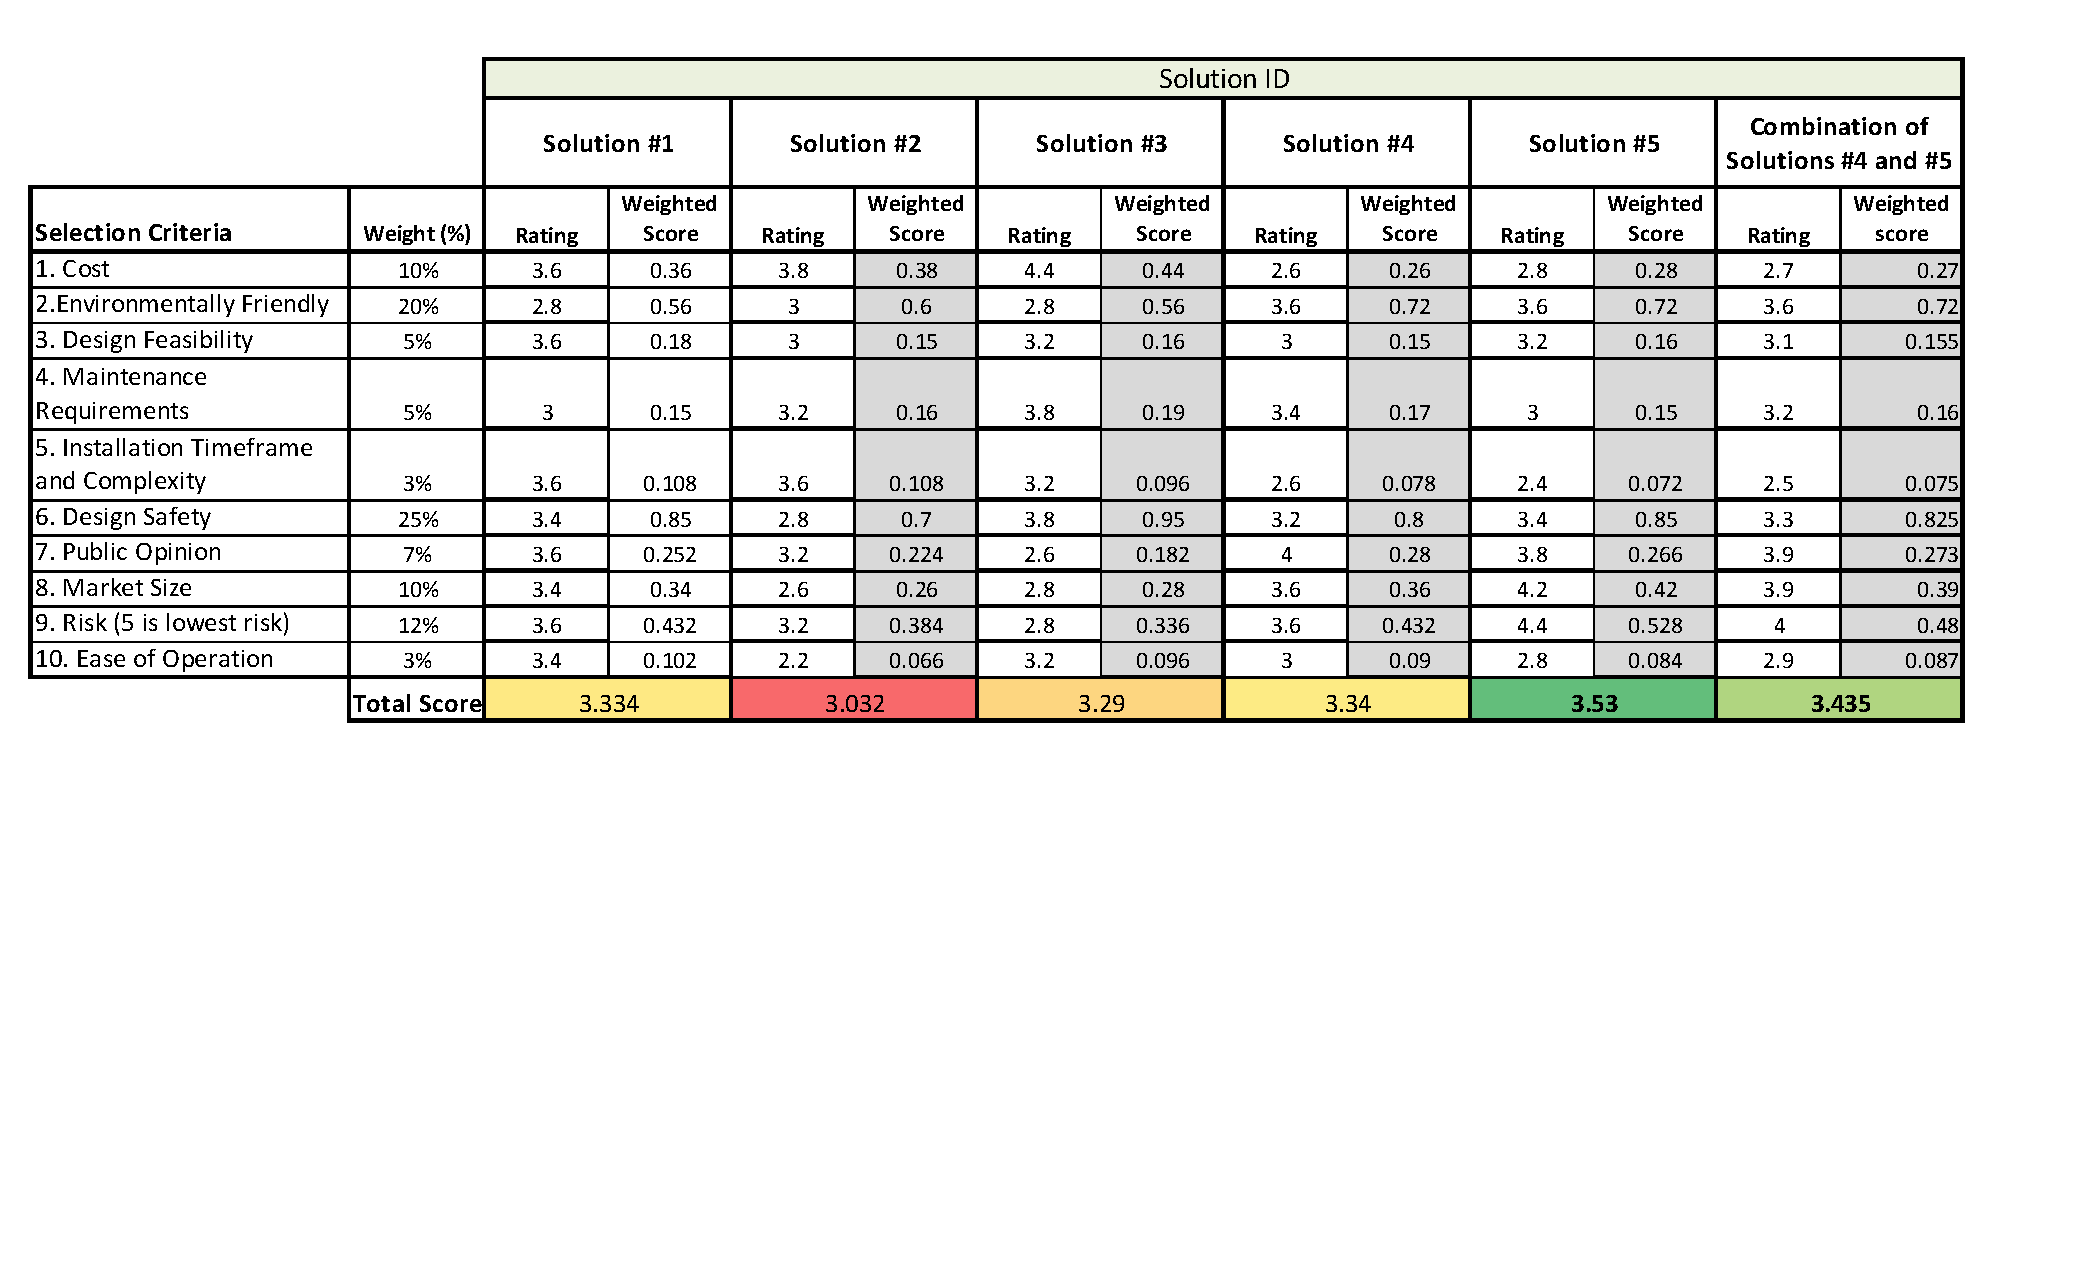
\includegraphics[width = 7.5in, angle = -90]{selectionMatrixV2.pdf}}
\caption{Prototype Selection Matrix}
\label{fig:selectionMatrix}
\end{figure}
\FloatBarrier

\newpage
After completing the decision matrix (as seen above in Figure \ref{fig:selectionMatrix}), the team came to the conclusion that we should incorporate several of the solutions since the concepts were mostly independent of each other (note the column "Combination of Solution 4 and 5). The main takeaway from the exercise was that the team favored the private hangar solution over the universal hangar. We found that it was a more marketable solution with less complications logistically as comapared to a power generation system or subsidy package.\par 
The team then discussed the value of the remaining solutions and decided to move forward with all four of them in some capacity. We believed that they could complement each other in order to create a broader process of transitioning every facet of an airport to accomaodate electric aircraft. Having come to this conclusion, we decided to set our focus on creating guidelines for an airport to make this transition. We acknowledged that this would exclude us from more material/technical prototypes, but we felt that this was the most interesting and promising path forward.\par
The team then began the prototype phase and conceptualized the guidelines through a storyboard (via PowerPoint) and a flowchart that acts as a roadmap of considerations for the airports. We went through several different versions of each prototype in order to restructure our most promising pieces and continue to improve the design. We also received feedback from our research partner, Bill Grauer, on the flowchart prototype, which will be featured in the discussion of said prototype below.\par

\newpage
\subsection{Storyboard representation of the selected prototype}
This section displays our storyboard prototype in an easily understood graphical format through the usage of a storyboard. The storyboard walks through the current challenges that we face with our environment and how our solution, the consultation toolkit, will aid airports in the future to incorporate electric aircraft solutions. We decided that a storyboard would be helpful because it breaks down our detailed solution into a more digestable format for our target market to look at and understand the full scope of our problem.\par

\begin{figure}
\centering
\fbox{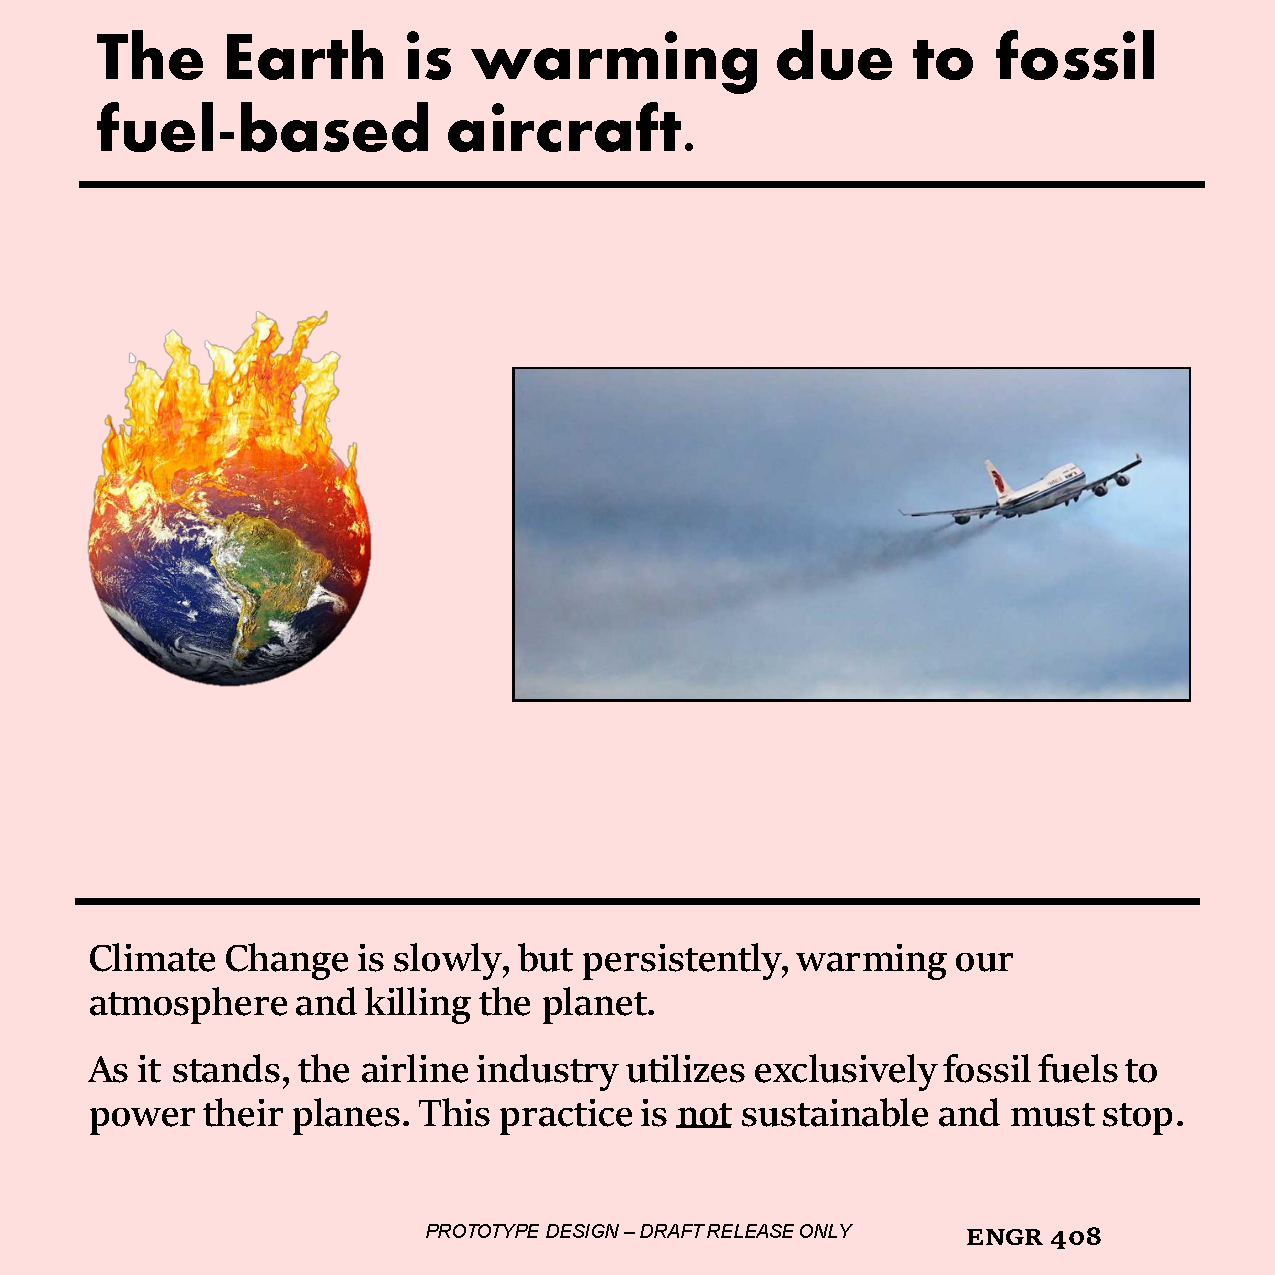
\includegraphics[width = \sbWidth]{SB1.pdf}}
\caption{Solution Storyboard}
\end{figure}
\newpage

\begin{figure}
\centering
\fbox{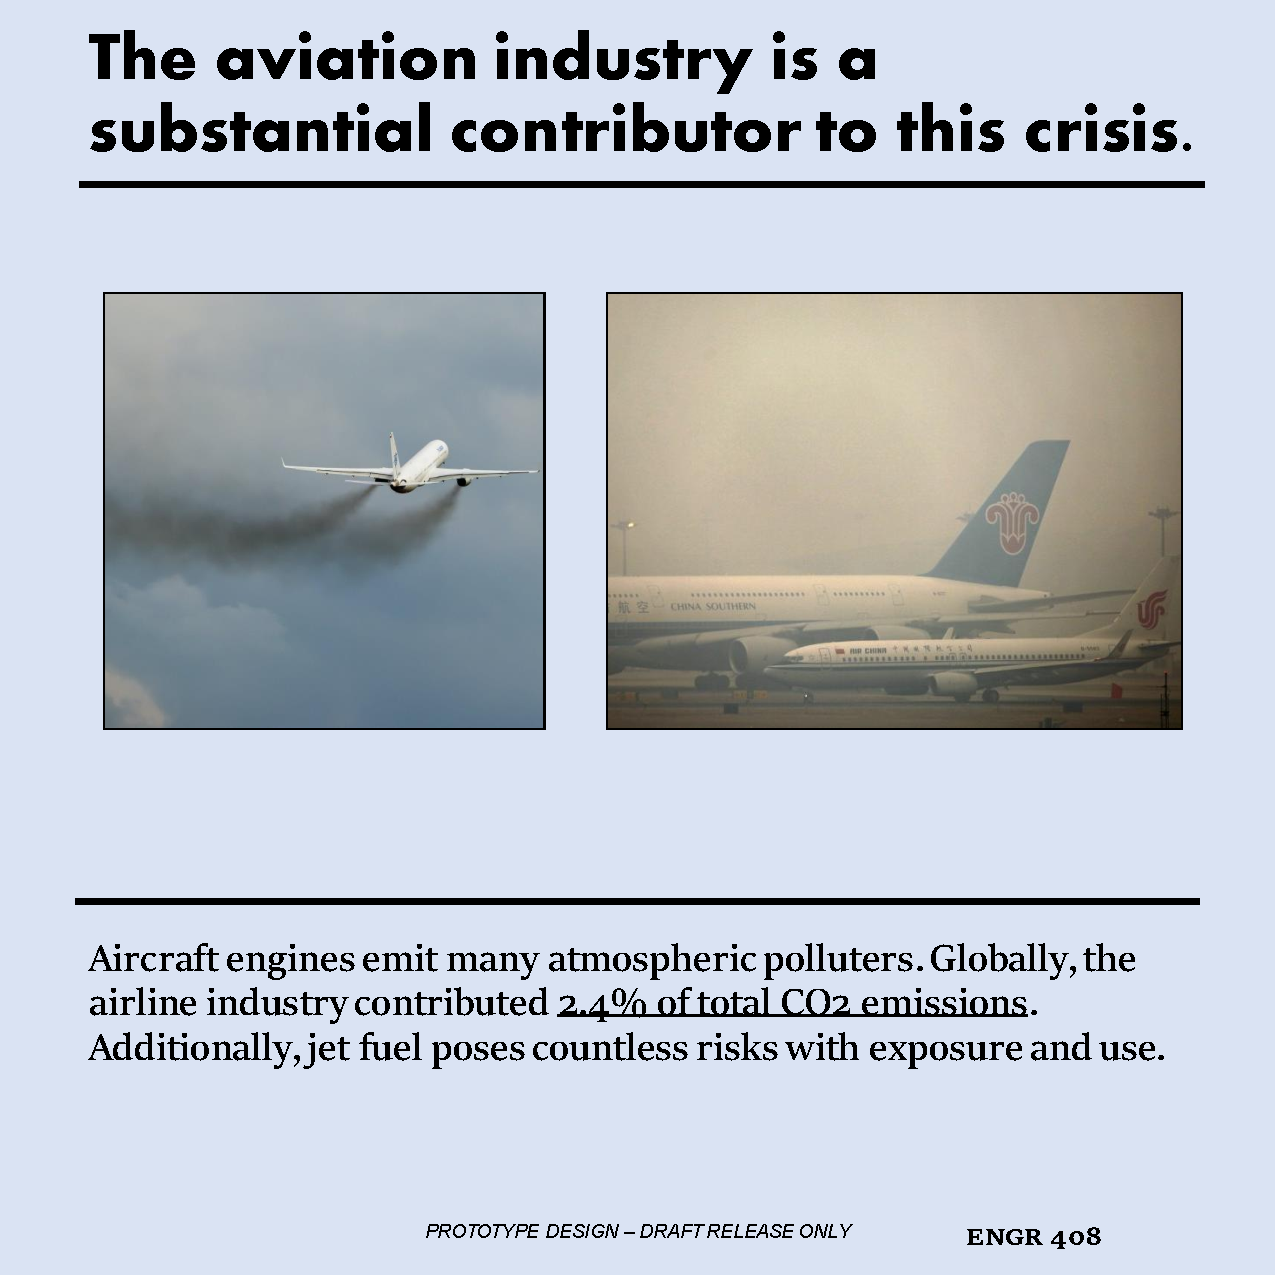
\includegraphics[width = \sbWidth]{SB2.pdf}}
\caption{Solution Storyboard}
\end{figure}
\newpage

\begin{figure}
\centering
\fbox{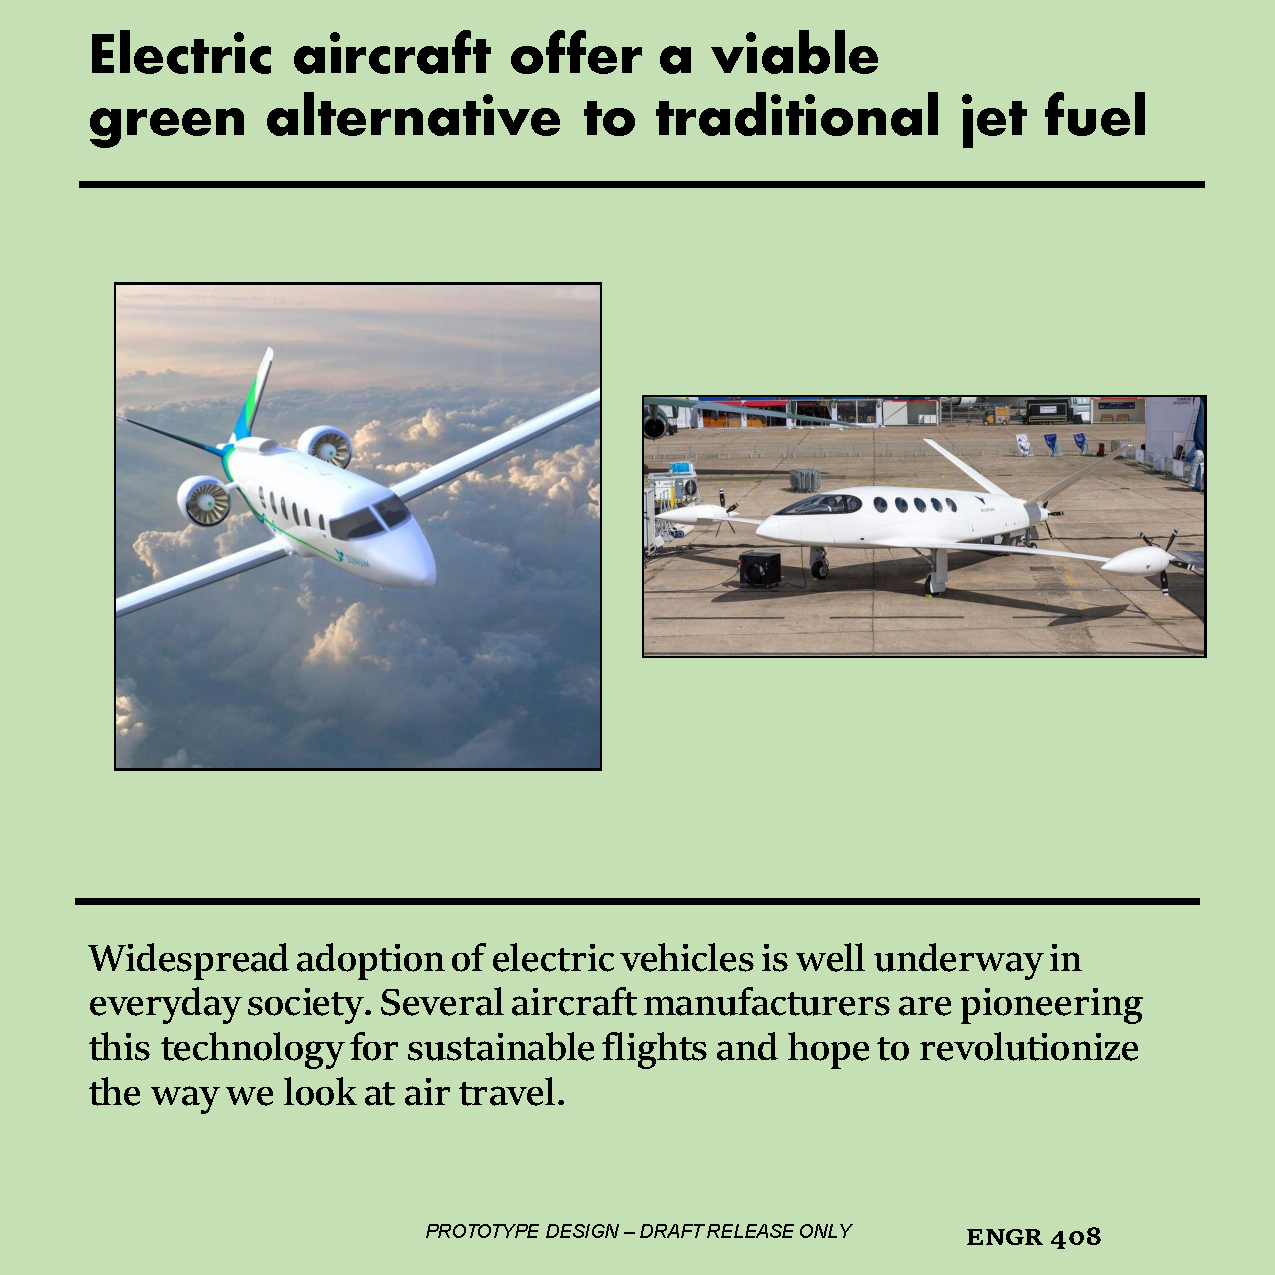
\includegraphics[width = \sbWidth]{SB3.pdf}}
\caption{Solution Storyboard}
\end{figure}
\newpage

\begin{figure}
\centering
\fbox{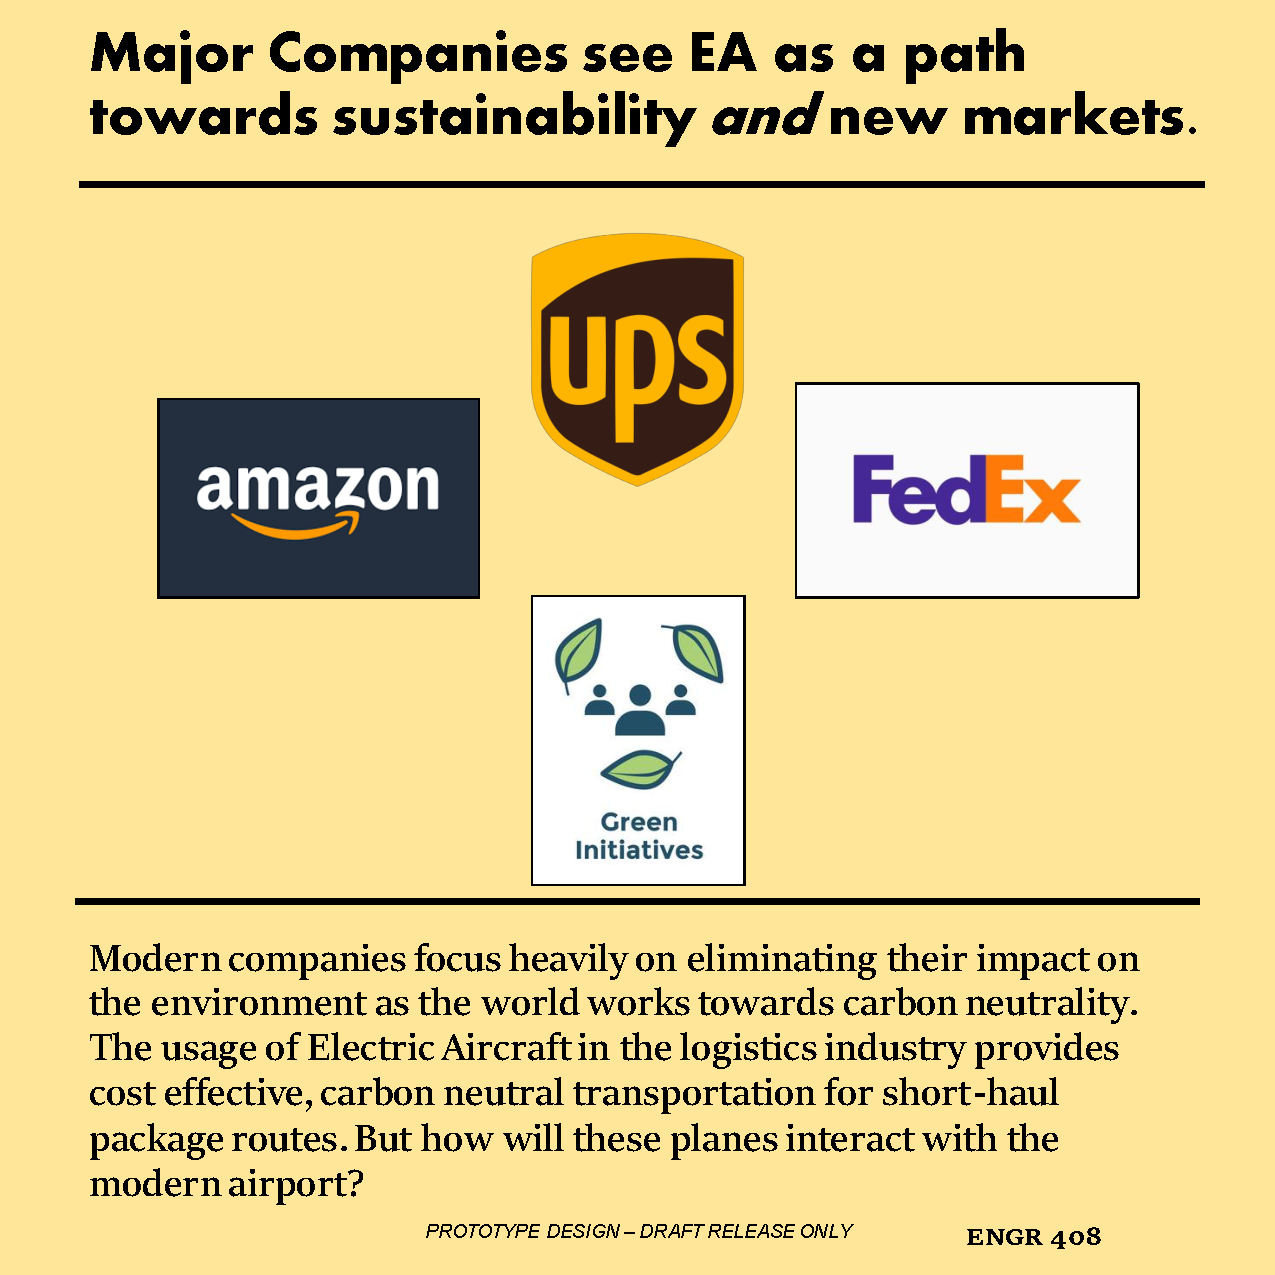
\includegraphics[width = \sbWidth]{SB4.pdf}}
\caption{Solution Storyboard}
\end{figure}
\newpage

\begin{figure}
\centering
\fbox{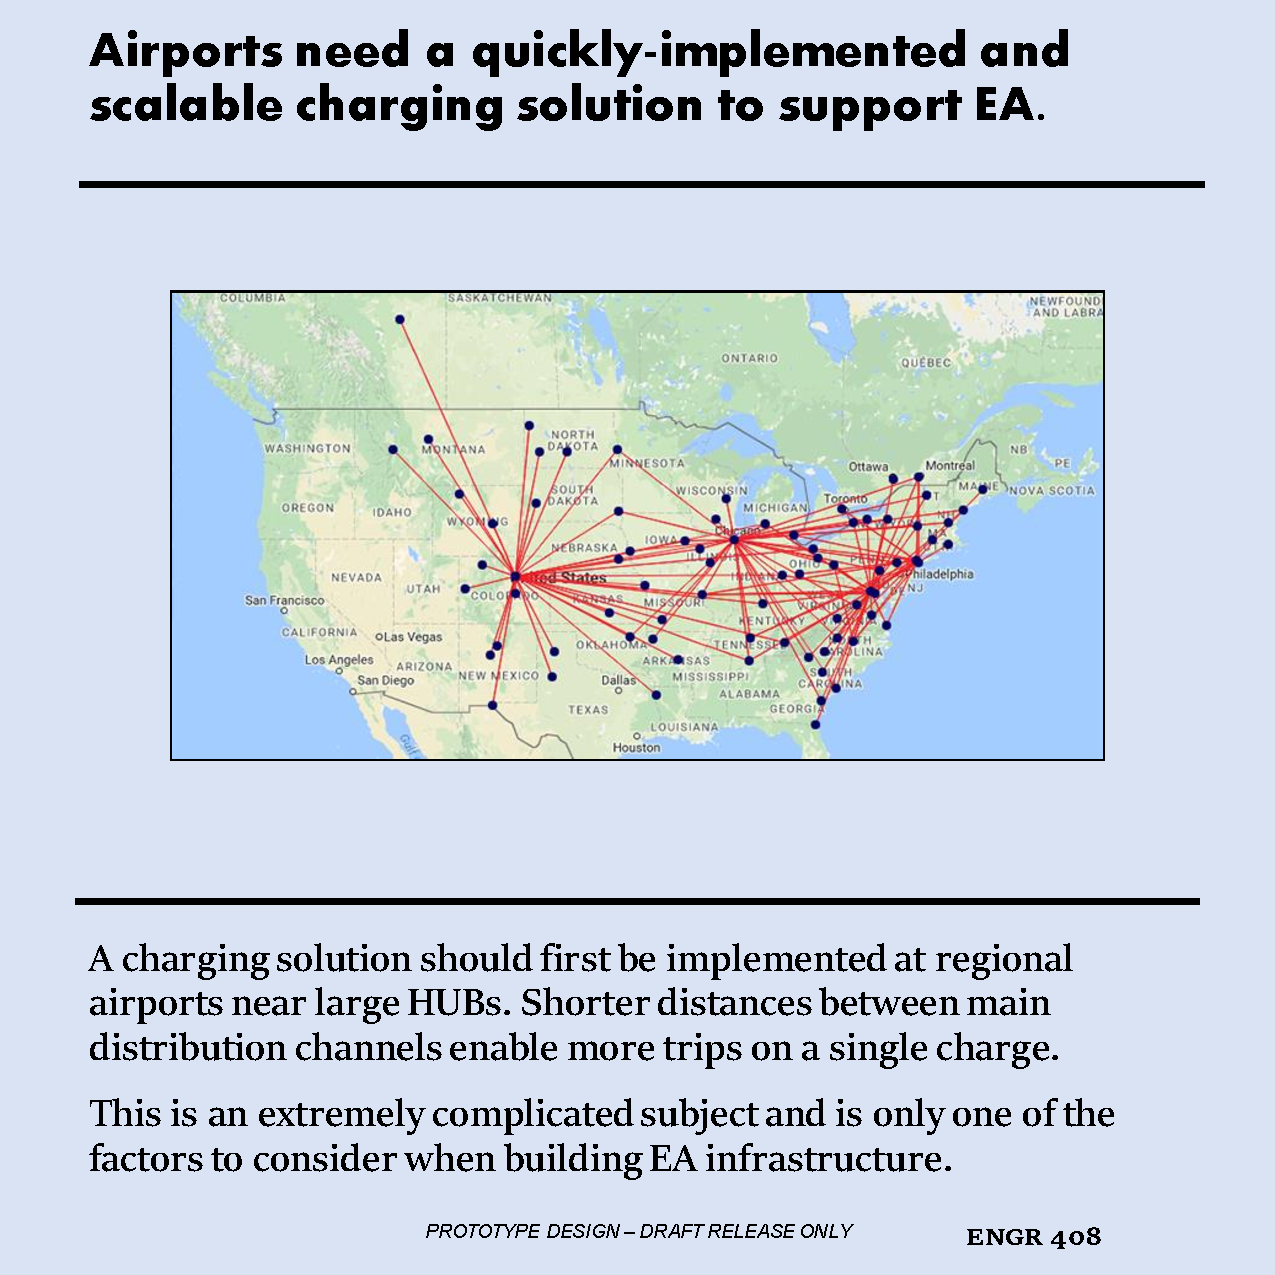
\includegraphics[width = \sbWidth]{SB5.pdf}}
\caption{Solution Storyboard}
\end{figure}
\newpage

\begin{figure}
\centering
\fbox{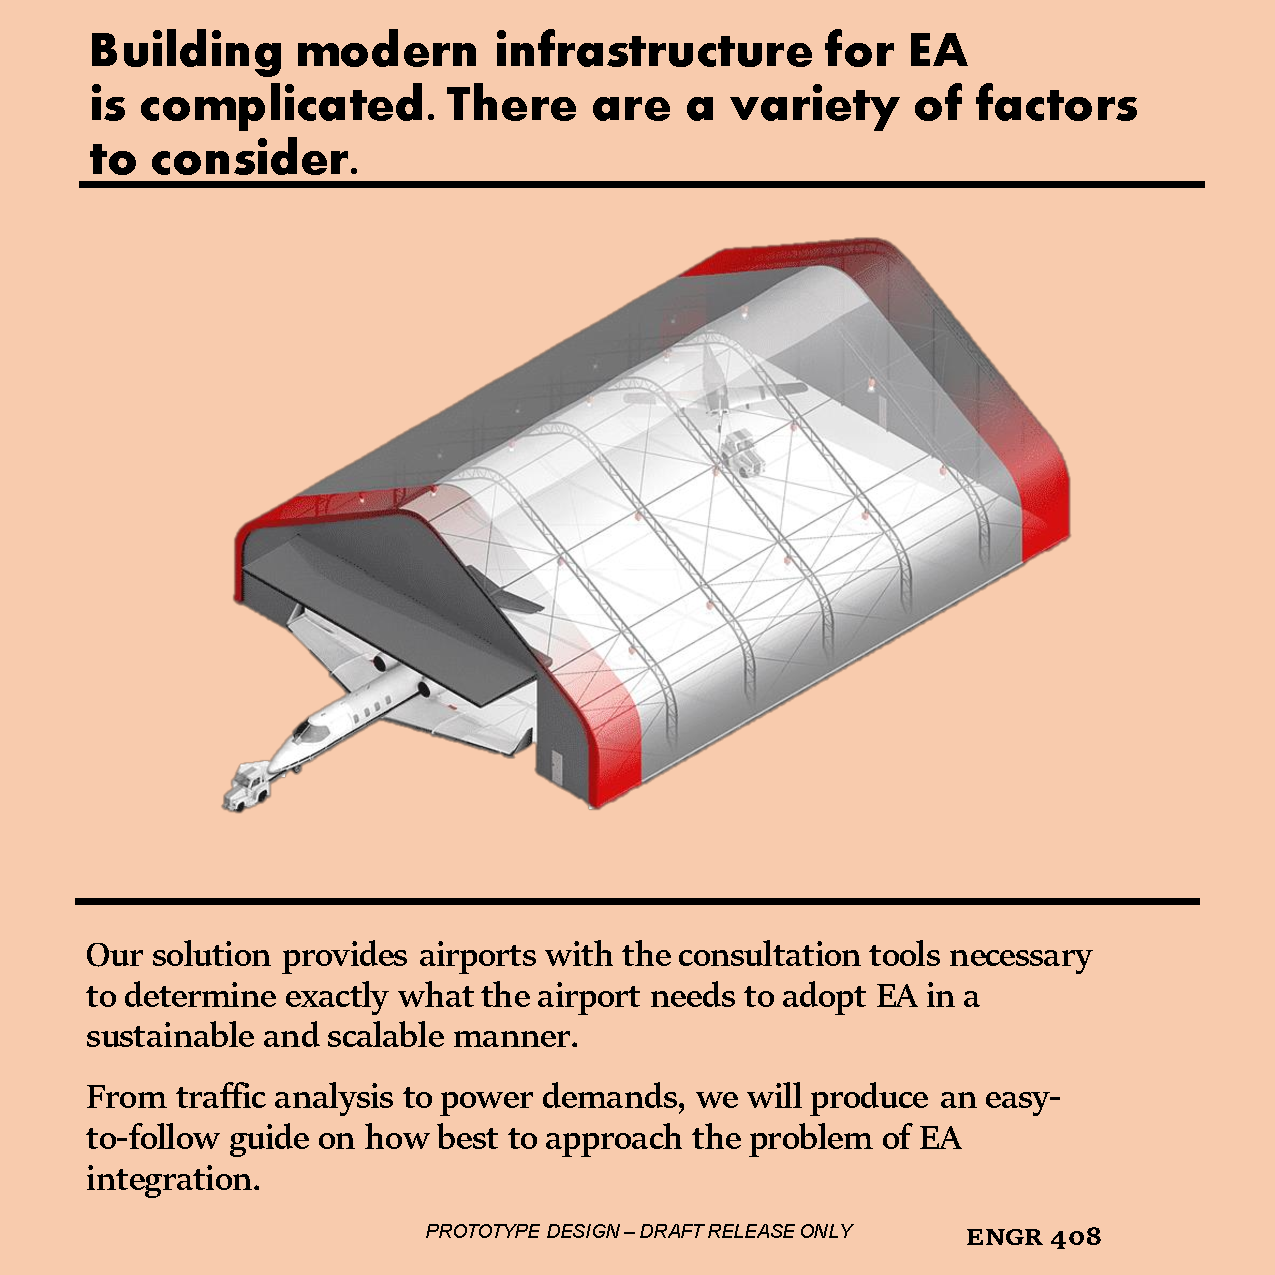
\includegraphics[width = \sbWidth]{SB6.pdf}}
\caption{Solution Storyboard}
\end{figure}
\newpage

\begin{figure}
\centering
\fbox{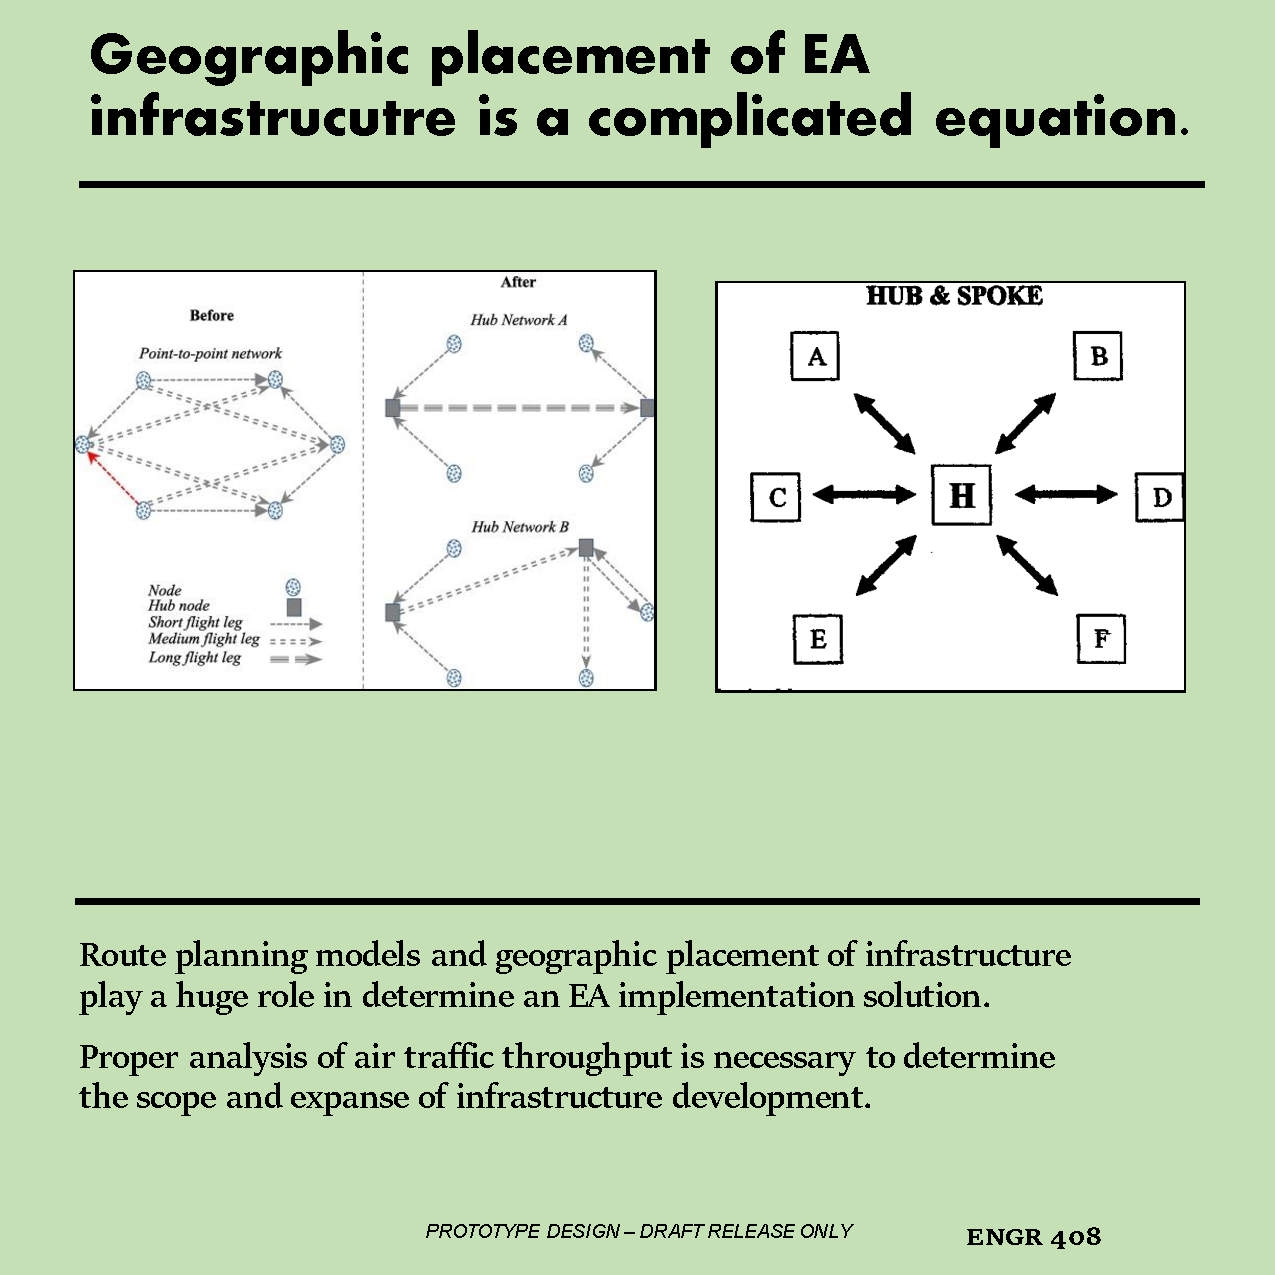
\includegraphics[width = \sbWidth]{SB7.pdf}}
\caption{Solution Storyboard}
\end{figure}
\newpage

\begin{figure}
\centering
\fbox{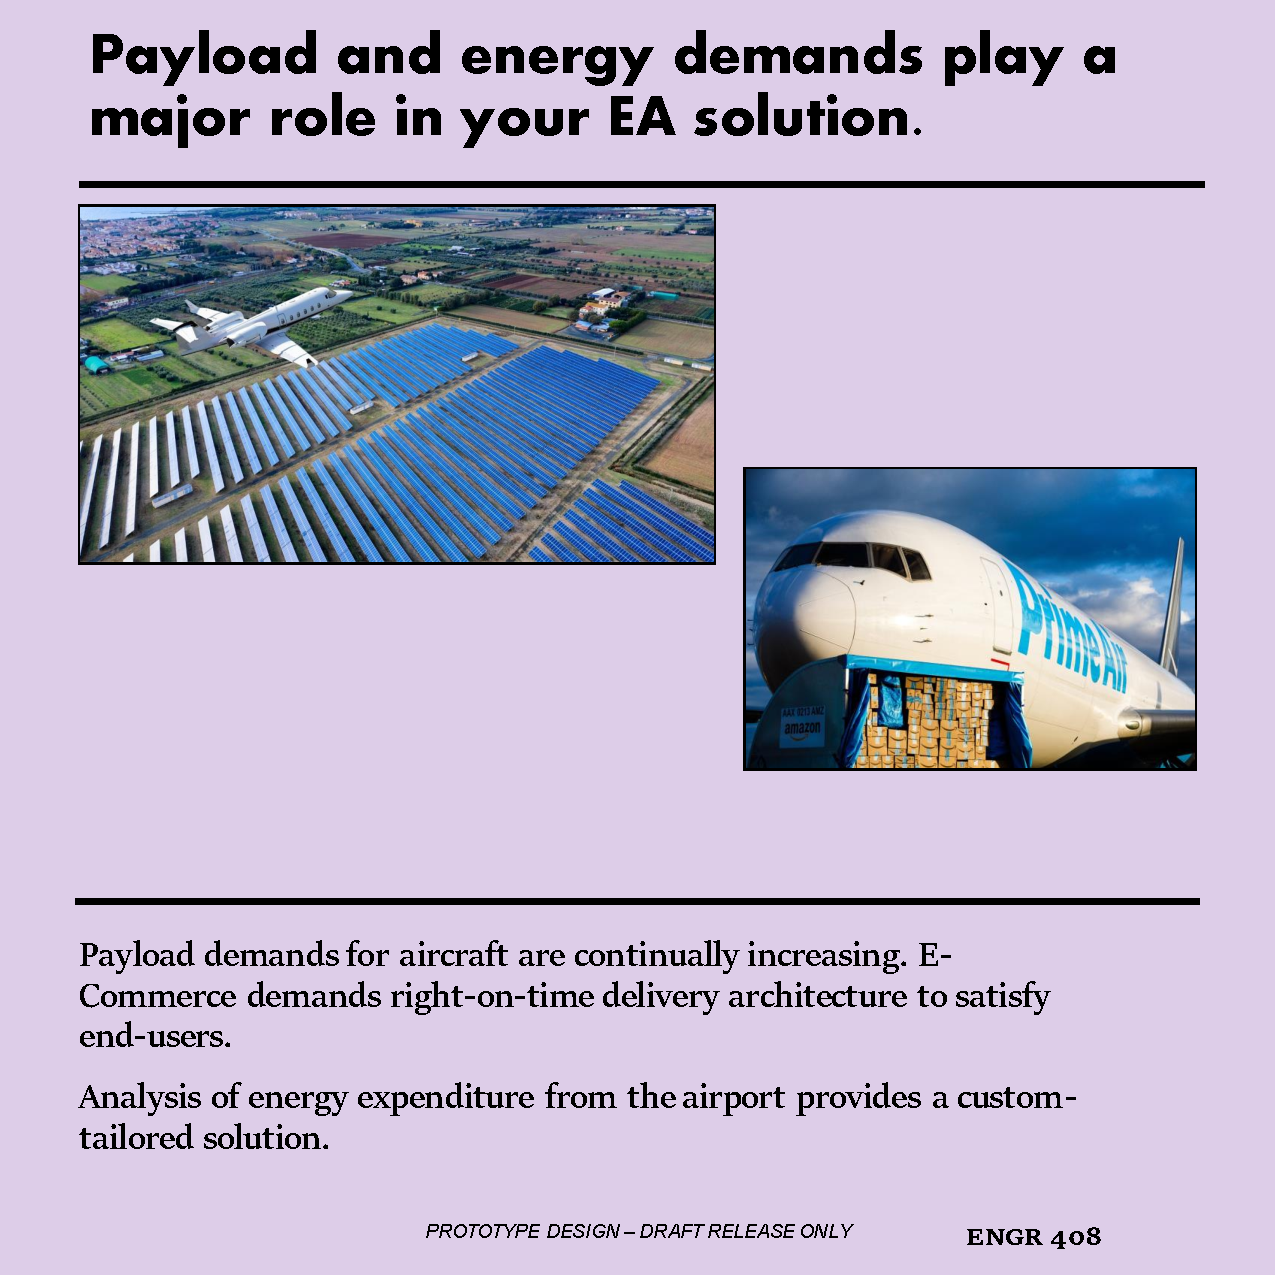
\includegraphics[width = \sbWidth]{SB8.pdf}}
\caption{Solution Storyboard}
\end{figure}
\newpage

\begin{figure}
\centering
\fbox{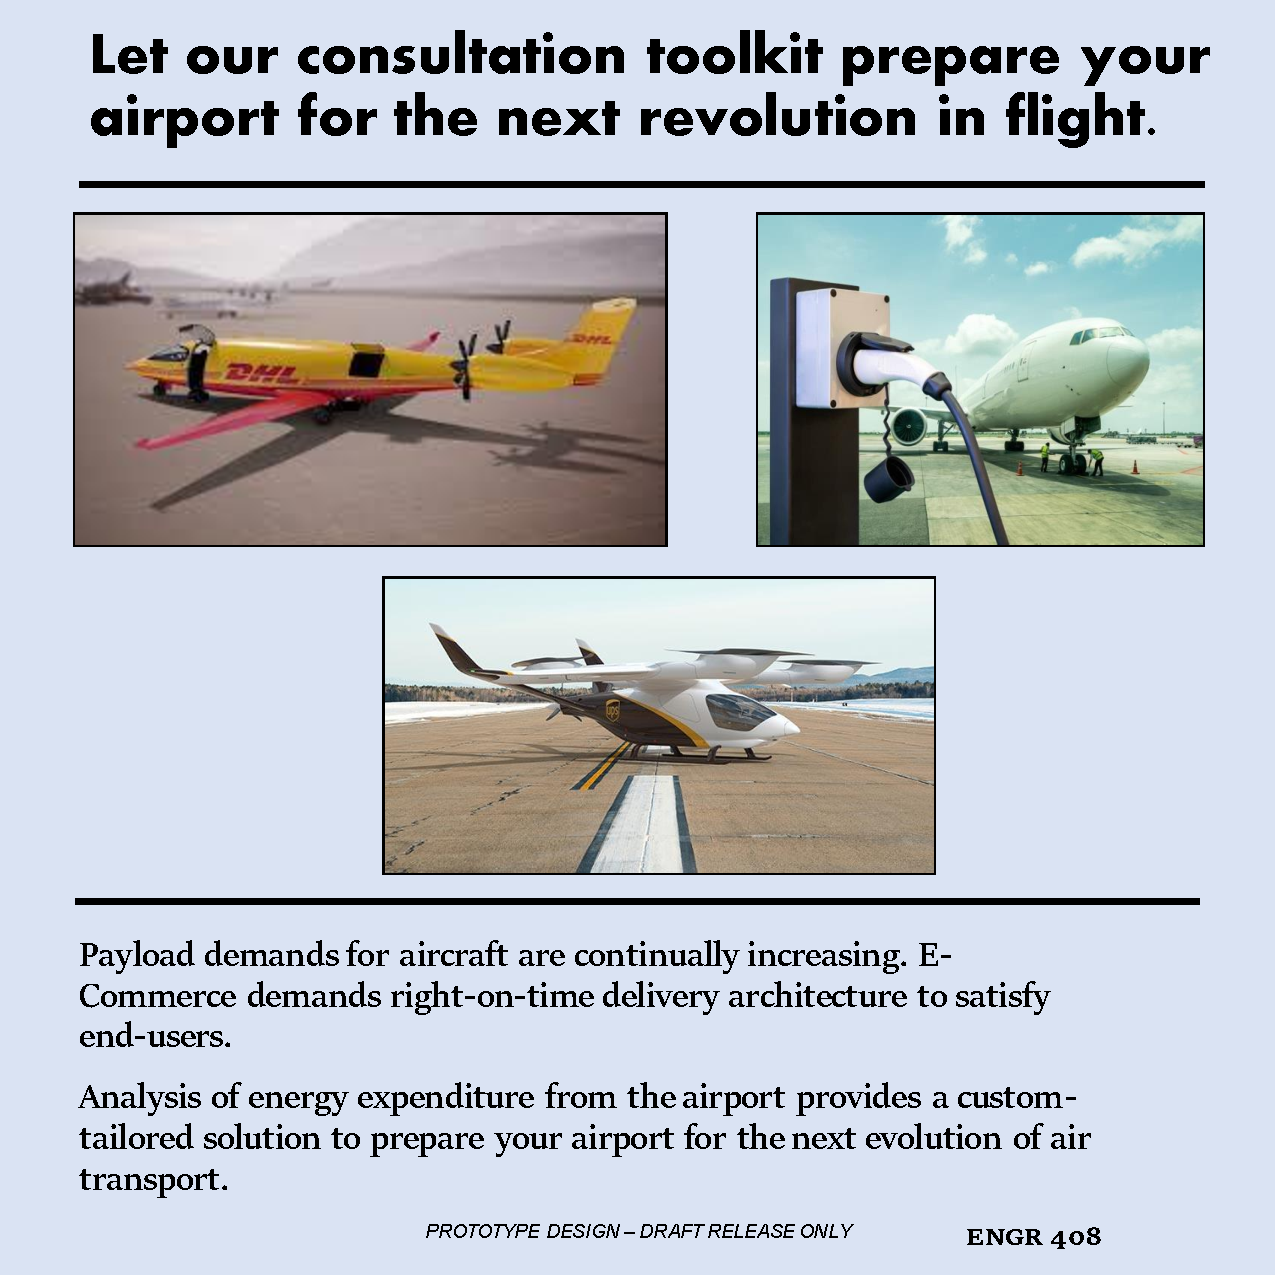
\includegraphics[width = \sbWidth]{SB9.pdf}}
\caption{Solution Storyboard}
\end{figure}
\FloatBarrier

\newpage
\subsection{Roadmap Prototype}
This section deatils our working Roadmap prototype and the process used to synthesize the map. The roadmap is a general guideline for airports that we hope to coordinate in an effort to seamlessly transition them into the world of electric aircraft as an EA-adoption toolkit. There are several areas of consideration that the roadmap explores, and we will further explain the sub-processes within this section of the report.\par
Below in Figure \ref{fig:roadmap} is the roadmap itself:\par

\begin{figure}[h!]
    \centering
    \fbox{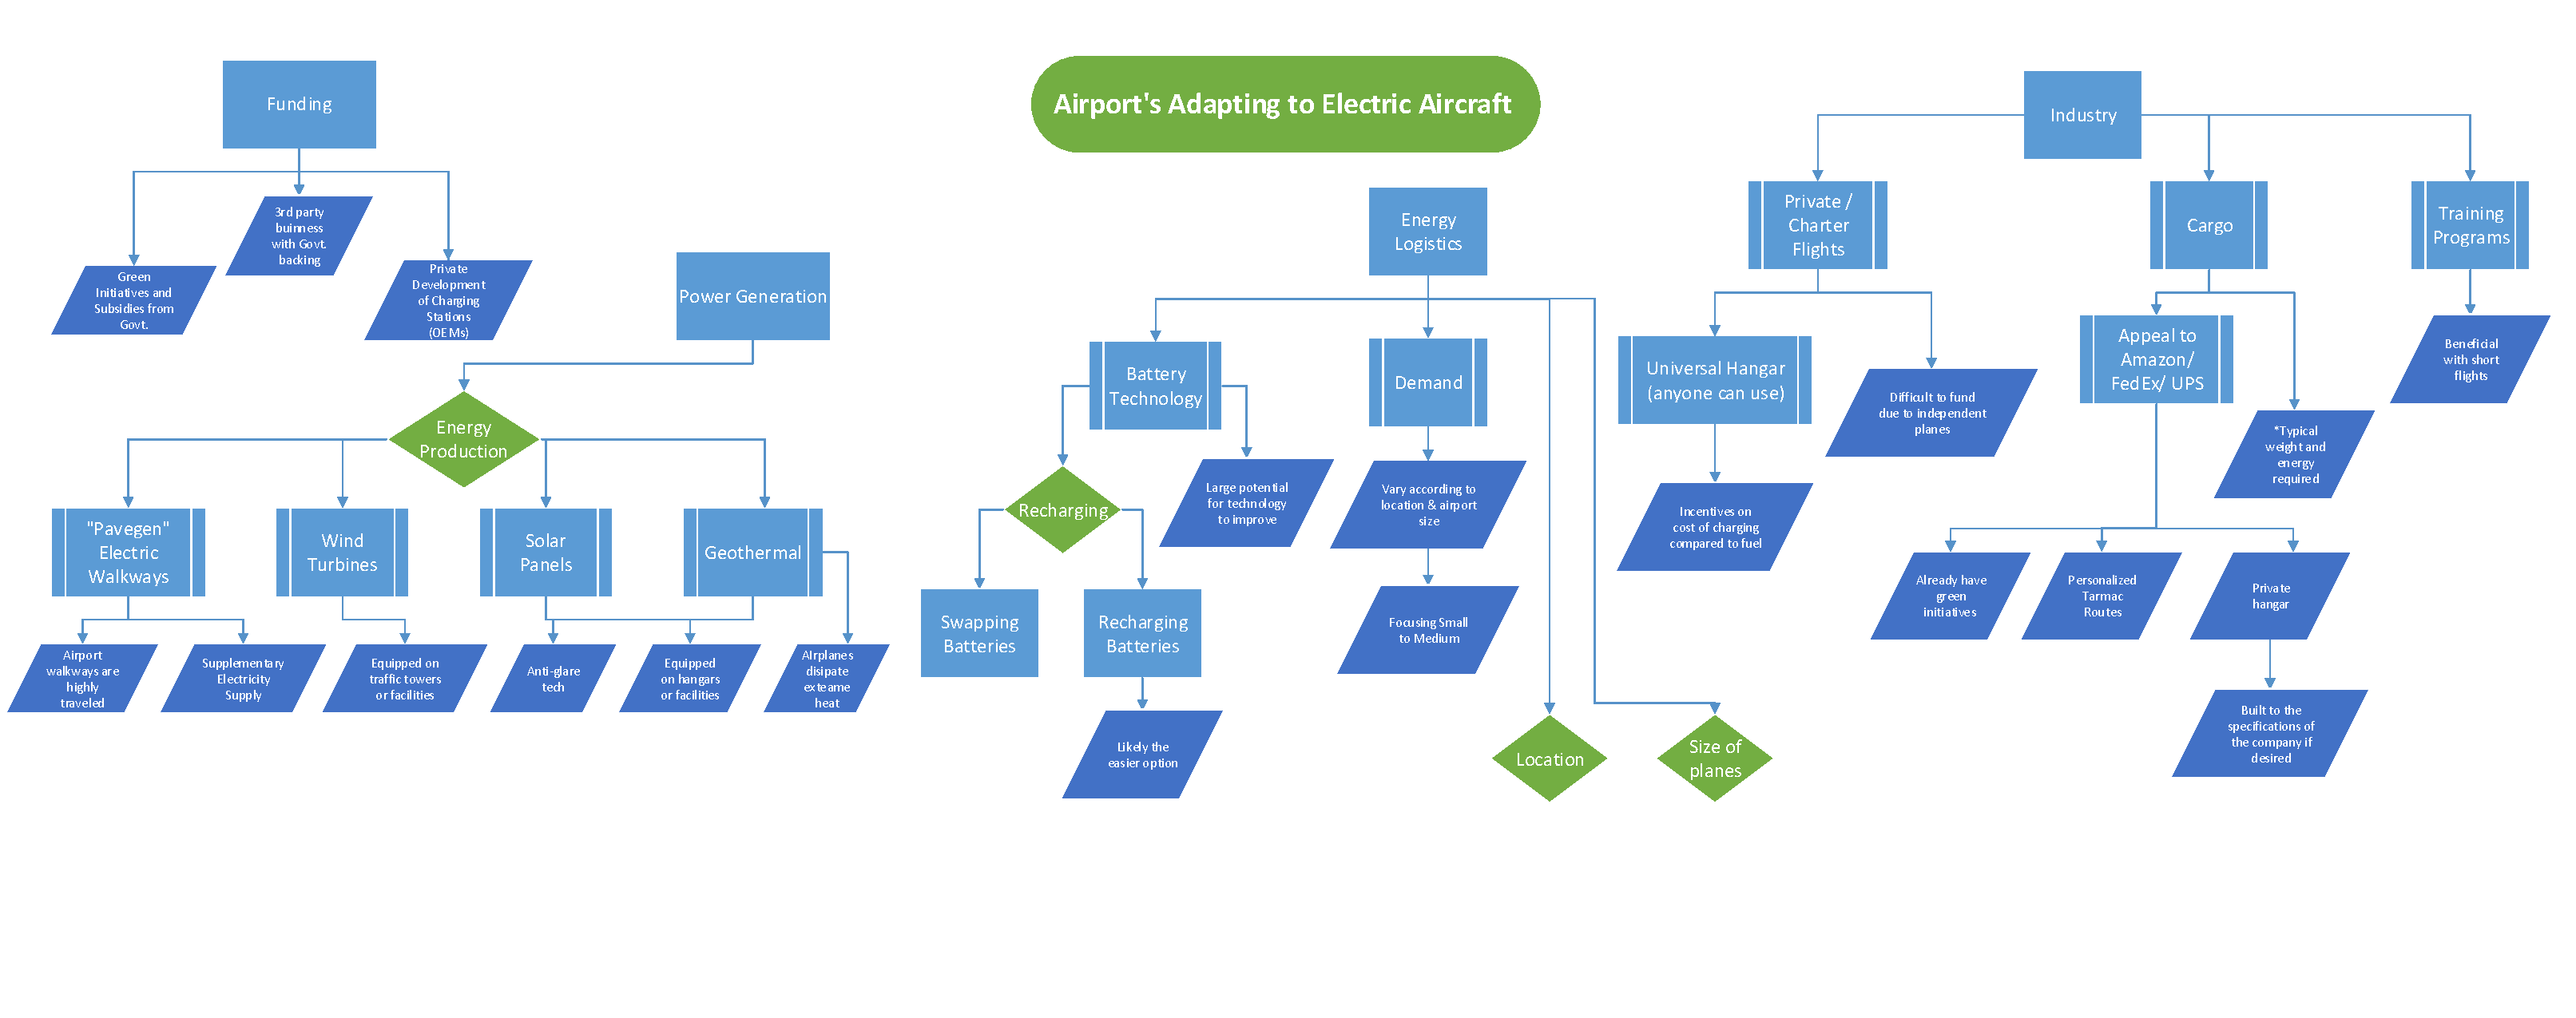
\includegraphics[width=\sbWidth]{Roadmap_Draft_D.pdf}}
    \caption{General guidelines to coordinate a seamless transition to an EA airport}
    \label{fig:roadmap}
    \centering
\end{figure}
\FloatBarrier

\subsubsection{Funding}
The first branch for our roadmap explores the funding for our solution. Funding is the one of the largest hurdles to overcome in our proposed solution--obtaining the capital required to implement the advanced infrastructure. This is also the area where we received the most feedback from our research partner Bill Grauer. He was fundamental in our understanding of how this solution's business model would have to be structured so that it can seamlessly integrate itself into the current-generation airports in a way that actually generates revenue for the system operators.\par 
Through this prototype, we are proposing the creation of a small 3rd party company that would obtain funding for the project and carry out the integration and implementation of the infrastructure at various airports. This avoids the convoluted nature of the airports having to raise the funding for the project privately or via convoluted capitol investment avenues. In order to convince the governments to fund the project, we would highlight the extremely low risk nature of investing in green energy generation and power storage at airports.\par
In the case that electric planes take off in the coming decades, the airport is already ahead of the curve on having the mandatory infrastructure for electric plane charging. In the case that electric planes take \emph{far longer} to come into the mainstream, the airports would still have power generation onsite to reduce the cost of electricity, or even sell off excess electricity if excess energy is created on site. The large energy storage system also provides a much stronger electric grid with a larger capacity, in which the government would eventually have had to invest anyway as time goes on and energy demands increase nationwide. Governments are the perfect candidate for this because of their ability to invest large amounts of money into projects for the common good, and because the government own in part or in full, most airports across the country.\par  
\newpage
\subsubsection{Power Generation}
In this section of the prototype, there are four main green energy generation sources.\par
The first and the most viable option currently is anti-glare solar panels. These panels, ideally, would be fastened on top of electric airplane hangars to receive the most sun exposure and help produce energy to recharge the electric planes. The available “anti-glare” technology would allow pilots to still land safely with the added benefit of absorbing more sunlight due to the coating.\par
Our second power generation prototype is wind turbines. These could be installed on the already built communication and signal towers or on adjacent buildings/structures. In theory, there would be smaller turbines in greater amounts that would aid the production of green energy. There is also the possibility of including larger turbines, but these would need to be strategically placed in order to avoid physical interference with the aircraft.\par
Our third option and the hardest to implement would be geothermal tarmacs; a large portion of energy dissipated from planes comes from the friction (heat) between the tires and the tarmac. Each plane taking off-- and even more so landing-- would contribute to this power generation technique. \par
Lastly, our fourth option-- which is intended to be more of a supplement to the established larger power generation solution-- is compression based electric walkways. These walkways, popularly referred to as “Pavegen” due to the leading company, works by generating electricity from each step taken on the walkway. As airports feature a lot of high foot-traffic areas, the walkways would turn these passenger routes into green energy. Although this is not a huge producer of energy, each tile creates about 2-4 joules per step - not an insignificant amount of energy considering the foot traffic present at an airport.
\newpage
\subsubsection{Energy Logistics}
In this section of the prototype, we explored the logistics of the energy infrastructure in relation to battery technology. We detail the different options in the recharging of aircraft through swapping the batteries or recharging them within the plane. We believe that recharging will be the favorable option as you don't have to pull out the entire battery to do so. The second aspect to consider in our prototype was the demand that these aircraft are going to place on the infrastructure. This will, of course, vary with the size of the airport, but we want to focus on servicing small to medium range aircraft. Our power generation considerations will have to complement this aspect, especially since airport electrical grids are typically near maximum capacity.\par
We also considered the logistics of location and size for these aircraft. In the short term, we are looking at small to medium cargo and private aircraft. Due to the longer time between flights of these planes and their smaller size, modern battery technology can be implemented in these aircraft much sooner. This would allow the customer to get more value out of their investment in EA infrastructure sooner -- greatly strengthening our business model.\par
It would also be important to initially focus on rural areas that have a need for a stronger power grid, as they would be more inclined to implement our product. As time goes on, we would explore areas with stronger power grids, and large cargo and commercial planes. This is more feasible in the future due to the development of battery technology. In the future we are likely to see massive leaps in the energy density of batteries, and the speed at which they can charge. 

\newpage
\subsubsection{Industry receipt of the prototype}
The final consideration for the roadmap is the industry in question. We laid out a few general considerations that would have slight implications for the electrification of the airport. These industries of interest are private/charter, training programs, and cargo. At the same time, we recognize that the private/charter industry would be difficult to fund since there are many independent aircraft that would not have the common interest of EA. The training programs are also a small industry, but we felt they were worth mentioning since the flights are typically small distances that would be perfect for an electric aircraft's battery.\par
The most promising aspect of the airport industry is cargo. Our prototype would appeal to large delivery companies like Amazon, UPS, DHL, Fedex, etc. in order to provide them with a means of green air transport. This can help meet these companies environmental goals of becoming carbon neutral. Our prototype also recognizes that we should market to this industry with priority tarmac routes and private hangars equipped with several charging stations. 

\newpage
\end{document}